\appendix
\section{Comparison with the closest prior work}
\label{app:delineation}
Table~\ref{tab:delineation} lists what each close neighbour established and what our design adds.
\begin{table*}[h]
\small
\centering
\begin{tabular}{p{3.6cm}p{9.6cm}}
\toprule
\textbf{Closest neighbour} & \textbf{What it established / what it does not cover} \\
\midrule
XBCP \citep{a2606_15345} & Deep-research agents on BrowseComp-Plus with the corpus translated into 12 languages; oracle decomposition into retrieval vs integration. Question always English; query language never logged or forced; no Indic language; translated rather than native evidence. \\
MarathiWeb \citep{kale2026marathiweb} & Two web-search LLMs on native Marathi queries; failures attributed to integration by inspection. One language; evidence availability observed, not manipulated; no parallel English arm. \\
MAST Indic track \citep{mast2026} & Nine Indic query languages over the English BrowseComp-Plus corpus. English-only corpus, so the evidence-side gap is zero by construction; a systems shared task. \\
DELTA \citep{a2601_02956} & Names the gold-availability prior and regresses it out of single-shot RAG. No agent, no Indic, statistical rather than experimental control. \\
Where's Waldo \citep{a2610_00606} & Query-language preference with fixed paired context when a fact exists in one edition only; Bengali worst. No retrieval, no agent, no search-query language. \\
Diagnosing search failures \citep{a2608_01913} & Retrieval gap vs utilisation gap with oracle evidence. English only; the retrieval gap is not split into query formulation vs corpus coverage. \\
Cross-Lingual Cost \citep{a2507_07543}; XRAG \citep{a2505_10089}; tRAG/CrossRAG \citep{a2504_03616}; CORAL \citep{a2604_25676} & Query-language vs document-language effects in RAG; one controlled Google ablation; an agent that picks the corpus language. Non-agentic or end-accuracy only; no Indic; no decomposition. \\
\bottomrule
\end{tabular}
\caption{Novelty delineation. Comparison with the closest prior work.}
\label{tab:delineation}
\end{table*}

\section{All paired contrasts}
\label{app:contrasts}
Table~\ref{tab:fullcontrasts} lists every paired contrast for both languages and all four models.
\begin{table*}[p]\centering\scriptsize
\resizebox{\textwidth}{!}{
\begin{tabular}{p{5.6cm}llllllll}
\toprule
Contrast (percentage points) & \multicolumn{2}{c}{Gemini 2.5 Flash-Lite} & \multicolumn{2}{c}{Gemini 3.1 Flash-Lite} & \multicolumn{2}{c}{Gemini 3.6 Flash} & \multicolumn{2}{c}{Qwen3-30B-A3B} \\
 & Hindi & Telugu & Hindi & Telugu & Hindi & Telugu & Hindi & Telugu \\
\midrule
Total gap: English minus Indic question (free, both pools) & \textbf{+9.4 [+4.5, +14.3]$^{*}$} & +4.7 [-1.6, +11.0] & +3.0 [-2.0, +8.0] & +1.0 [-5.1, +7.1] & +2.0 [-4.0, +8.0] & -6.0 [-14.0, +0.0] & \textbf{+9.1 [+3.8, +14.6]$^{*}$} & +2.4 [-4.7, +9.4] \\
Recovered by dual-language queries & +1.8 [-3.2, +6.8] & -2.5 [-9.2, +4.2] & +1.0 [-4.0, +6.0] & -3.0 [-10.1, +3.0] & +0.0 [-6.0, +6.0] & -2.0 [-8.0, +4.0] & +4.5 [+0.7, +8.4]$^{*}$ & +3.9 [-0.8, +9.4] \\
Recovered by English-only queries & +4.5 [+0.0, +9.1] & +0.0 [-6.3, +6.3] & +2.0 [-3.0, +7.0] & -1.0 [-6.1, +4.0] & +6.0 [+0.0, +14.0] & -2.0 [-10.0, +6.0] & -1.4 [-6.3, +3.5] & -1.6 [-7.1, +3.9] \\
Recovered by matched-language queries & +0.7 [-3.1, +4.9] & -7.9 [-14.2, -1.6]$^{*}$ & +1.0 [-3.0, +6.1] & -2.0 [-6.1, +2.0] & -- & -- & +0.3 [-2.8, +3.5] & -0.8 [-6.3, +4.7] \\
Evidence-side: both pools minus English-only pool & -0.7 [-5.6, +3.8] & -1.6 [-7.9, +4.7] & -2.0 [-7.0, +3.0] & +1.0 [-3.0, +5.1] & +0.0 [-6.0, +6.0] & +2.0 [-6.0, +10.0] & +5.6 [+1.0, +10.5]$^{*}$ & +2.4 [-3.1, +7.9] \\
Evidence-side: both pools minus Indic-only pool & +0.3 [-3.5, +4.2] & +3.1 [-2.4, +8.7] & +4.0 [-2.0, +10.1] & +0.0 [-6.1, +6.1] & -- & -- & +1.4 [-1.7, +4.9] & +3.9 [-2.4, +11.0] \\
English queries minus matched queries, English-only pool & +6.3 [+1.7, +11.2]$^{*}$ & +2.4 [-3.1, +7.9] & +3.0 [-2.0, +8.0] & +3.0 [-2.0, +8.0] & -- & -- & +3.8 [-0.7, +8.7] & +2.4 [-4.7, +8.7] \\
English queries minus matched queries, Indic-only pool & -4.9 [-10.5, +0.3] & +0.8 [-7.1, +8.7] & +0.0 [-5.0, +5.0] & +1.0 [+0.0, +3.0] & -- & -- & -4.2 [-8.4, +0.0] & -7.1 [-14.2, +0.0] \\
Symmetric monolingual: en/en minus L/L & \textbf{+10.1 [+4.5, +15.7]$^{*}$} & +12.6 [+3.9, +21.3]$^{*}$ & -- & -- & -- & -- & \textbf{+13.2 [+7.7, +19.2]$^{*}$} & +3.1 [-4.7, +11.0] \\
Integration gap: oracle passage, English minus Indic question & \textbf{+6.3 [+2.8, +9.8]$^{*}$} & +6.3 [+0.0, +12.6] & -2.0 [-6.0, +2.0] & -1.0 [-5.0, +2.0] & -2.0 [-10.0, +4.0] & -2.0 [-6.0, +0.0] & +4.2 [+0.7, +7.7]$^{*}$ & +6.3 [+1.6, +11.0]$^{*}$ \\
Closed-book gap & +3.1 [-1.0, +7.7] & +3.9 [-2.4, +11.0] & +3.0 [-4.0, +10.0] & -1.0 [-7.0, +5.0] & +2.0 [-4.0, +8.0] & +0.0 [-6.0, +6.0] & \textbf{+12.9 [+7.3, +18.5]$^{*}$} & +7.1 [+0.0, +14.2] \\
Total gap under BM25 & \textbf{+18.9 [+12.9, +24.8]$^{*}$} & +11.0 [+2.4, +19.7]$^{*}$ & -- & -- & -- & -- & \textbf{+19.5 [+13.6, +25.8]$^{*}$} & \textbf{+14.2 [+6.3, +22.0]$^{*}$} \\
Symmetric monolingual under BM25 & \textbf{+35.3 [+29.0, +42.0]$^{*}$} & \textbf{+31.0 [+20.6, +41.3]$^{*}$} & -- & -- & -- & -- & -- & -- \\
Recovered by dual queries under BM25 & \textbf{+9.3 [+3.9, +14.6]$^{*}$} & +7.6 [-1.7, +16.8] & -- & -- & -- & -- & \textbf{+13.6 [+8.4, +18.8]$^{*}$} & +9.4 [+2.4, +17.3]$^{*}$ \\
Indic question: BM25 minus dense (free, both) & \textbf{-15.7 [-21.3, -10.1]$^{*}$} & \textbf{-21.3 [-30.7, -12.6]$^{*}$} & -- & -- & -- & -- & \textbf{-16.0 [-21.6, -10.5]$^{*}$} & \textbf{-18.9 [-28.3, -9.4]$^{*}$} \\
\midrule
Policy $\times$ evidence interaction & \textbf{+11.2 [+4.2, +18.2]$^{*}$} & +1.6 [-7.9, +11.0] & +3.0 [-4.0, +10.0] & +2.0 [-3.0, +8.0] & -- & -- & +8.0 [+2.1, +14.3]$^{*}$ & +9.4 [+0.0, +18.9] \\
\bottomrule
\end{tabular}}
\caption{Paired within-item contrasts (percentage points) with item-bootstrap 95\% intervals. $^{*}$: sign-flip permutation $p<0.05$. Bold: survives Benjamini--Hochberg over the full family of 144 tests (threshold $p \le 0.0076$). Positive total gap = the English question is answered more often. Dense retriever unless marked BM25.}
\label{tab:fullcontrasts}
\end{table*}
\section{Additional figures}
\begin{figure*}[h]\centering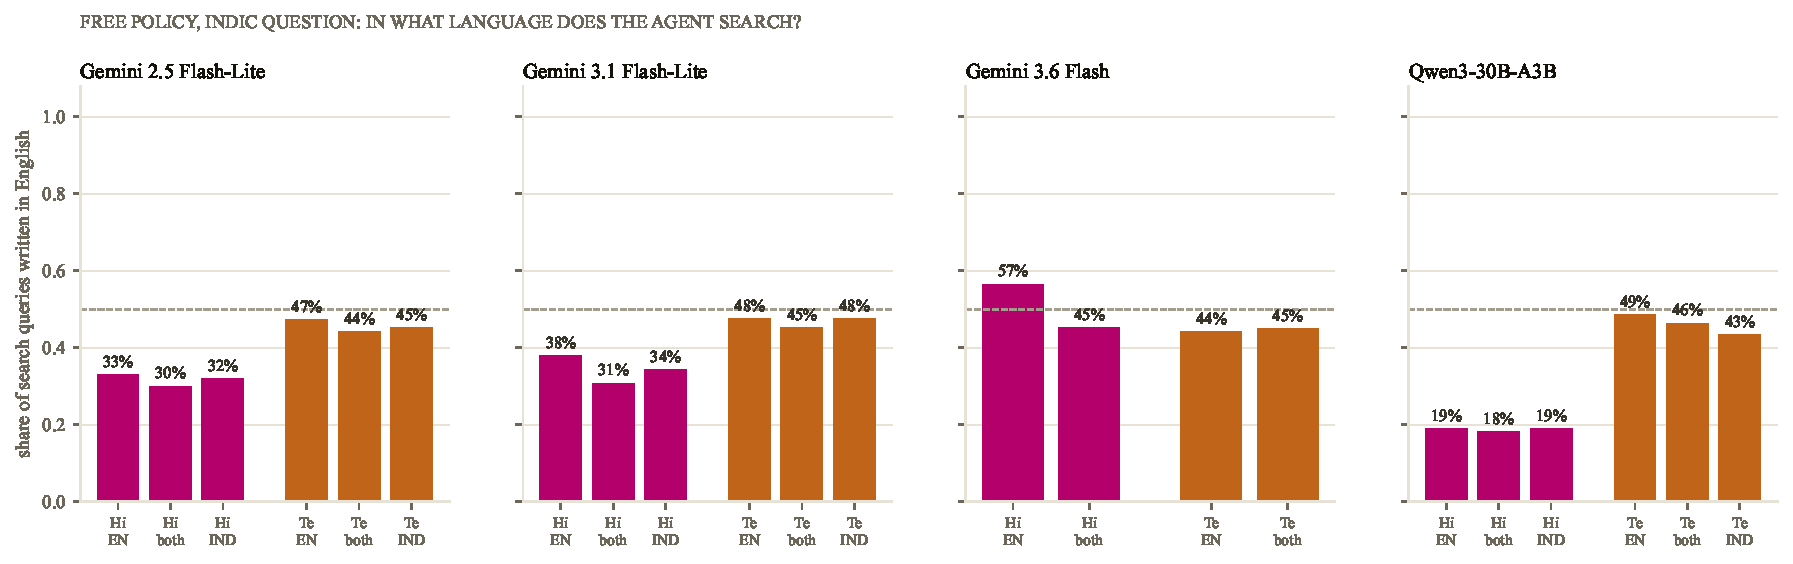
\includegraphics[width=0.8\textwidth]{assets/fig2_query_language.pdf}
\caption{Share of search queries written in Latin script when the question is in Hindi (magenta) or Telugu (orange), free policy, by served pool (EN = English-only, IND = Indic-only). Dashed line: one half.}\label{fig:fig2}\end{figure*}
\begin{figure*}[h]\centering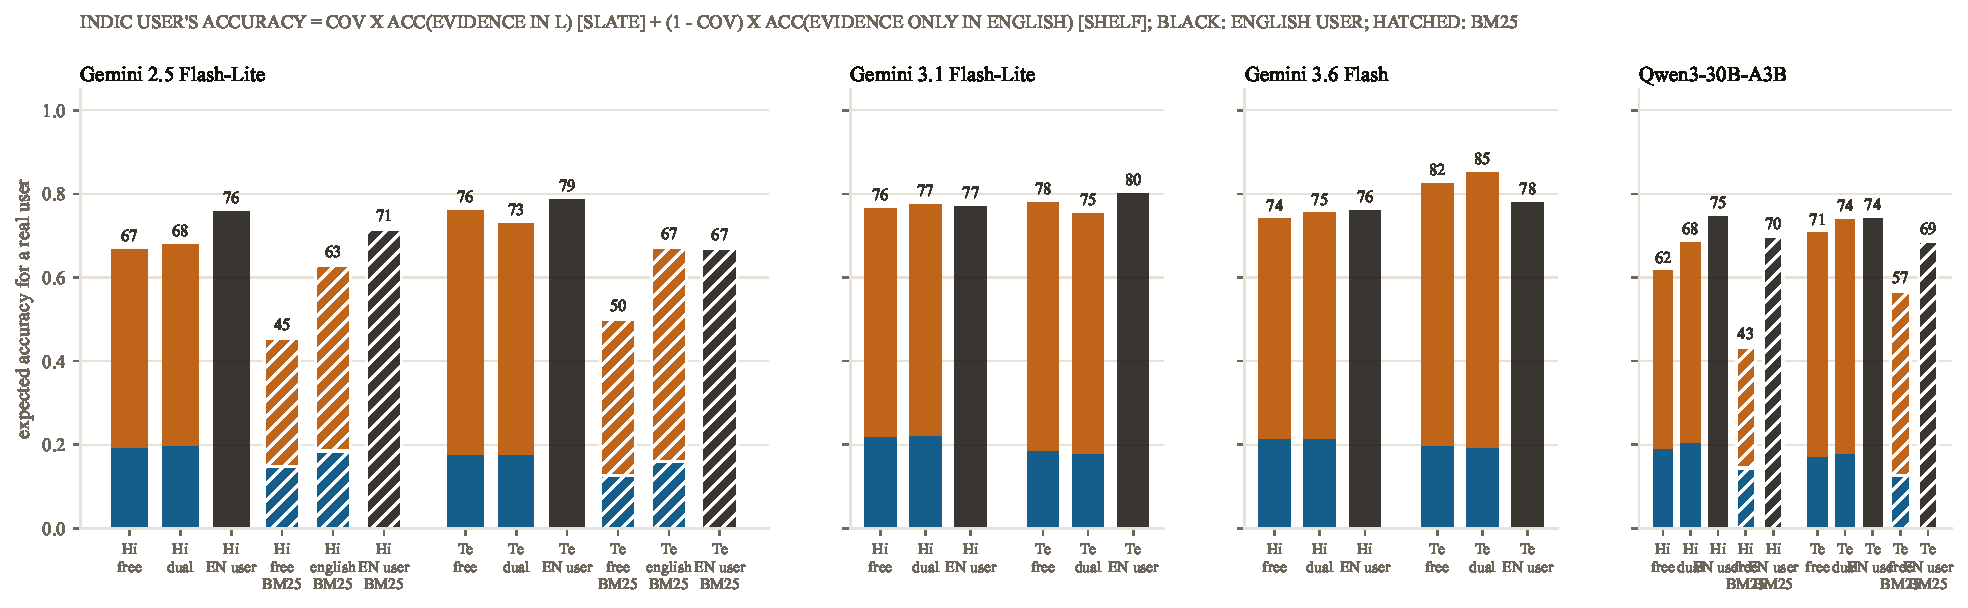
\includegraphics[width=0.85\textwidth]{assets/fig4_decomposition.pdf}
\caption{Expected accuracy of a real Indic user from Eq.~\ref{eq:decomp}: the slate part is coverage times accuracy with evidence in both languages; the orange part is the remaining share times accuracy on the English-only pool; black is the English user. Hatched bars use BM25.}\label{fig:fig4}\end{figure*}
\begin{figure}[h]\centering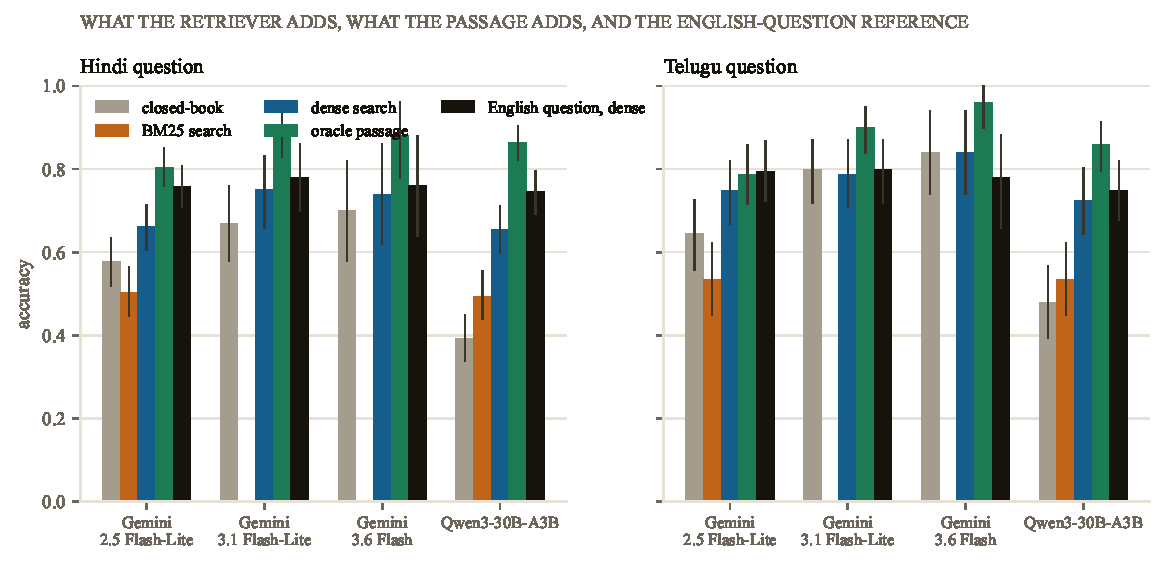
\includegraphics[width=\columnwidth]{assets/fig5_retriever_oracle.pdf}
\caption{Indic question, free policy, both pools: closed-book, BM25 search, dense search, gold passage in the prompt, and the English question with dense search, per model.}\label{fig:fig5}\end{figure}
\section{Verbatim prompts and tool schema}
\label{app:prompts}

All prompts are reproduced exactly as sent. The policy sentence is appended to the system prompt; \texttt{\{qlang\}} is the name of the question's language and \texttt{\{max\_searches\}}=3, \texttt{\{k\}}=5.

\paragraph{Agent system prompt}
\begin{quote}\small\ttfamily\raggedright
You are a search agent. You answer factual questions by searching a document collection with the `search` tool, reading the returned passages, and then giving a short final answer. \par Rules: \par - You may call `search` at most \{max\_searches\} times. Each call returns the top \{k\} passages. \par - When you have enough evidence, or when you have used all your searches, stop calling tools and reply with the final answer only: a short phrase (a name, date, number, or term), no explanation. \par - Answer in the same language as the question. \par - If the evidence does not contain the answer, you may still answer from your own knowledge, but prefer the evidence.\{policy\}
\end{quote}

\paragraph{Policy sentence: free}
\begin{quote}\small\ttfamily\raggedright
(none)
\end{quote}

\paragraph{Policy sentence: match}
\begin{quote}\small\ttfamily\raggedright
- Write every search query in \{qlang\}, the language of the question.
\end{quote}

\paragraph{Policy sentence: english}
\begin{quote}\small\ttfamily\raggedright
- Write every search query in English, even though the question is in \{qlang\}. Translate the information need into an English query.
\end{quote}

\paragraph{Policy sentence: dual}
\begin{quote}\small\ttfamily\raggedright
- At every step call `search` twice: once with a query in \{qlang\} (the language of the question) and once with the same information need as an English query. Both calls count as one step.
\end{quote}

\paragraph{Tool schema (JSON)}
\begin{quote}\small\ttfamily\raggedright
\{ \par  "type": "function", \par  "function": \{ \par   "name": "search", \par   "description": "Search the document collection. Returns the most relevant passages with their titles.", \par   "parameters": \{ \par    "type": "object", \par    "properties": \{ \par     "query": \{ \par      "type": "string", \par      "description": "The search query." \par     \} \par    \}, \par    "required": [ \par     "query" \par    ] \par   \} \par  \} \par \}
\end{quote}

\paragraph{Empty-result message}
\begin{quote}\small\ttfamily\raggedright
No passages found for this query.
\end{quote}

\paragraph{Closed-book system prompt}
\begin{quote}\small\ttfamily\raggedright
You answer factual questions from your own knowledge. Reply with the final answer only: a short phrase (a name, date, number, or term), no explanation. Answer in the same language as the question.
\end{quote}

\paragraph{Oracle system prompt}
\begin{quote}\small\ttfamily\raggedright
You answer a factual question using the passage provided. Reply with the final answer only: a short phrase (a name, date, number, or term), no explanation. Answer in the same language as the question.
\end{quote}

\paragraph{Oracle user message}
\begin{quote}\small\ttfamily\raggedright
Passage: \par """ \par \{passage\} \par """ \par  \par Question: \{question\}
\end{quote}

\paragraph{Judge system prompt}
\begin{quote}\small\ttfamily\raggedright
You are a strict grader of short answers to factual questions. Decide whether the candidate answer expresses the same fact as any of the gold answers. Accept equivalent forms: a transliteration or translation of the gold answer into another language or script, a date written differently, a number with or without units, a name with or without honorifics, a more specific answer that contains the gold answer. Reject answers that name a different entity, date, or number, that hedge between several candidates. If the candidate declines to answer, says the information is unavailable, or asks a question back, that is ABSTAIN.
\end{quote}

\paragraph{Judge user message}
\begin{quote}\small\ttfamily\raggedright
Question (English): \{q\_en\} \par Question (original): \{q\_L\} \par Gold answers: \{gold\} \par Candidate answer: \{cand\} \par  \par Reply with exactly one word: CORRECT, WRONG, or ABSTAIN (the candidate says it does not know, cannot find the answer, or asks for clarification instead of answering).
\end{quote}

\section{Coverage measurement and audit}
\label{app:coverage}
For each of the 539 XorQA-In test questions per language we resolved the English source article to its Hindi or Telugu counterpart through Wikidata sitelinks (916 of 918 distinct titles resolved; two had no Wikidata item) and looked the counterpart up in the 20261001 snapshot. An article exists for 364 Hindi and 283 Telugu items. Coverage was then decided in three steps. (1) \emph{String match}: the Indic gold answer, or the English gold answer, occurs in the article after NFC normalisation and punctuation stripping; 119 Hindi and 94 Telugu items (the 237 Telugu items whose released translated answer is the function word ``{\telu అని}'' were matched on the English answer only). (2) \emph{Two independent LLM reads}: gemini-2.5-flash-lite and then gemini-3.6-flash were each given the question in both languages, the gold answers and the full article (up to 14,000 characters) and asked to quote verbatim the sentence that states the answer or reply NONE; a read counts only if the quoted sentence is found in the article. The first read accepted 205 Hindi and 179 Telugu items; the second accepted 158 and 129; both agree on 157 and 127, which are the verified-coverage counts (29.1\% and 23.6\%). (3) \emph{Manual audit}: before the second read, we drew 25 items per language stratified over first-read outcomes and labelled them by reading the quoted sentence against the question. Of the 30 first-read acceptances, 21 were correct, 7 were uncertain (the quote did not visibly contain the answer) and 2 were wrong (the Hindi article gives 13 South American countries where the gold says twelve; the Telugu Gandhi article never names Subhas Chandra Bose). The second read rejected 1 of the 2 wrong, 4 of the 7 uncertain and 8 of the 21 correct acceptances, so the final coverage figure is conservative: it under-counts rather than over-counts. The 20 first-read rejections in the audit were not labelled by hand; the second read accepted 3 of them with a verbatim quote, but an item needs both reads to count, so they stay outside the controlled grid and the coverage figure. The audit file with every label is shipped as \texttt{results/coverage\_audit.json}.
\section{Judge audit}
\label{app:audit}
Of the judged agent answers, the string rule decided 41\% (exact or contained match to a gold alias in either script after digit normalisation); the rest went to the LLM judge (gemini-2.5-flash, not in the grid), which returned CORRECT, WRONG or ABSTAIN. We drew 40 judged answers (20 per language: 10 string-correct, 5 LLM-correct, 5 LLM-wrong or abstain) and labelled them by hand against the question and gold aliases. All 40 verdicts agreed with the manual label. Cases worth noting: a Korean-script answer accepted for the romanised gold ``mumu''; ``labour movement'' accepted for ``trade union movement''; an answer naming one of three states in the gold marked WRONG, which we consider defensible; and seven abstentions (``the search results do not contain\ldots'') marked ABSTAIN and scored as wrong. The sample is shipped as \texttt{results/audit\_sample.json}.
\section{Per-cell tables}
\label{app:cells}
\begin{table*}[h]\centering\scriptsize
\begin{tabular}{lllrrrrr}
\toprule
Question & Policy & Pool & n & Acc & 95\% CI & English queries & gold in top-5 \\
\midrule
Hindi & closed & (no tool) & 287 & 57.8 & [51.9, 63.4] & 0\% & 0\% \\
Hindi & dual & Indic-only & 281 & 61.9 & [56.2, 67.6] & 50\% & 79\% \\
Hindi & dual & Indic-only [bm25] & 280 & 34.3 & [28.6, 39.6] & 52\% & 20\% \\
Hindi & dual & both & 280 & 67.9 & [62.5, 73.6] & 50\% & 87\% \\
Hindi & dual & both [bm25] & 281 & 58.7 & [53.0, 64.4] & 51\% & 67\% \\
Hindi & dual & English-only & 280 & 67.9 & [62.1, 73.2] & 50\% & 83\% \\
Hindi & dual & English-only [bm25] & 280 & 58.2 & [52.5, 63.9] & 51\% & 61\% \\
Hindi & english & Indic-only & 287 & 61.3 & [55.7, 66.9] & 100\% & 68\% \\
Hindi & english & Indic-only [bm25] & 285 & 32.3 & [27.0, 37.9] & 100\% & 8\% \\
Hindi & english & both & 287 & 70.7 & [65.5, 76.0] & 100\% & 80\% \\
Hindi & english & both [bm25] & 287 & 63.4 & [57.8, 69.0] & 100\% & 63\% \\
Hindi & english & English-only & 287 & 70.7 & [65.5, 76.0] & 100\% & 80\% \\
Hindi & english & English-only [bm25] & 287 & 62.7 & [57.1, 68.3] & 100\% & 59\% \\
Hindi & free & Indic-only & 287 & 65.9 & [60.3, 71.4] & 32\% & 74\% \\
Hindi & free & Indic-only [bm25] & 287 & 40.1 & [34.5, 45.6] & 38\% & 17\% \\
Hindi & free & both & 287 & 66.2 & [60.6, 71.4] & 30\% & 79\% \\
Hindi & free & both [bm25] & 286 & 50.3 & [44.7, 56.3] & 28\% & 40\% \\
Hindi & free & English-only & 287 & 66.9 & [61.3, 72.5] & 33\% & 72\% \\
Hindi & free & English-only [bm25] & 286 & 43.4 & [37.8, 49.3] & 35\% & 38\% \\
Hindi & free & (gold hidden) & 49 & 55.1 & [40.8, 69.4] & 27\% & 0\% \\
Hindi & match & Indic-only & 286 & 66.4 & [60.8, 71.7] & 1\% & 74\% \\
Hindi & match & Indic-only [bm25] & 286 & 35.3 & [29.7, 40.9] & 1\% & 16\% \\
Hindi & match & both & 287 & 66.9 & [61.7, 72.5] & 1\% & 78\% \\
Hindi & match & both [bm25] & 287 & 43.6 & [38.0, 49.5] & 2\% & 23\% \\
Hindi & match & English-only & 286 & 64.3 & [58.7, 69.9] & 1\% & 66\% \\
Hindi & match & English-only [bm25] & 286 & 19.6 & [15.0, 24.5] & 2\% & 3\% \\
Hindi & oracle L & (gold passage) & 287 & 72.8 & [67.6, 78.0] & 0\% & 0\% \\
Hindi & oracle en & (gold passage) & 287 & 80.5 & [76.0, 85.0] & 0\% & 0\% \\
English & closed & (no tool) & 287 & 61.0 & [55.4, 66.6] & 0\% & 0\% \\
English & dual & Indic-only & 287 & 64.5 & [58.9, 70.0] & 97\% & 72\% \\
English & dual & Indic-only [bm25] & 287 & 25.8 & [20.9, 31.0] & 97\% & 8\% \\
English & free & Indic-only & 287 & 65.9 & [60.3, 71.1] & 100\% & 70\% \\
English & free & Indic-only [bm25] & 286 & 32.2 & [26.6, 37.8] & 100\% & 8\% \\
English & free & both & 286 & 75.9 & [71.0, 80.8] & 100\% & 83\% \\
English & free & both [bm25] & 287 & 69.0 & [63.4, 74.2] & 100\% & 65\% \\
English & free & English-only & 285 & 75.8 & [70.9, 80.7] & 100\% & 82\% \\
English & free & English-only [bm25] & 287 & 71.4 & [66.2, 76.7] & 100\% & 65\% \\
English & match & Indic-only & 287 & 64.8 & [59.2, 70.4] & 100\% & 70\% \\
English & match & Indic-only [bm25] & 287 & 38.3 & [32.8, 43.9] & 100\% & 8\% \\
English & match & both & 287 & 74.9 & [70.0, 79.8] & 100\% & 82\% \\
English & match & both [bm25] & 287 & 71.4 & [66.2, 76.7] & 100\% & 65\% \\
English & match & English-only & 287 & 76.3 & [71.4, 81.2] & 100\% & 82\% \\
English & match & English-only [bm25] & 287 & 70.7 & [65.5, 76.0] & 100\% & 64\% \\
English & oracle en & (gold passage) & 287 & 86.8 & [82.9, 90.6] & 0\% & 0\% \\
\bottomrule
\end{tabular}
\caption{All cells, Gemini 2.5 Flash-Lite, Hindi items (n = items; `English queries' = share of search calls written in Latin script; `gold in top-5' = share of episodes in which a gold chunk was retrieved).}
\end{table*}

\begin{table*}[h]\centering\scriptsize
\begin{tabular}{lllrrrrr}
\toprule
Question & Policy & Pool & n & Acc & 95\% CI & English queries & gold in top-5 \\
\midrule
Telugu & closed & (no tool) & 127 & 64.6 & [55.9, 72.4] & 0\% & 0\% \\
Telugu & dual & Indic-only & 118 & 71.2 & [62.7, 78.8] & 50\% & 81\% \\
Telugu & dual & Indic-only [bm25] & 118 & 44.9 & [35.6, 54.2] & 51\% & 13\% \\
Telugu & dual & both & 119 & 74.8 & [66.4, 82.4] & 50\% & 89\% \\
Telugu & dual & both [bm25] & 119 & 61.3 & [52.9, 69.7] & 50\% & 60\% \\
Telugu & dual & English-only & 119 & 72.3 & [63.9, 79.8] & 50\% & 89\% \\
Telugu & dual & English-only [bm25] & 118 & 54.2 & [44.9, 62.7] & 51\% & 55\% \\
Telugu & english & Indic-only & 127 & 67.7 & [59.1, 75.6] & 100\% & 65\% \\
Telugu & english & Indic-only [bm25] & 127 & 44.1 & [35.4, 52.8] & 100\% & 5\% \\
Telugu & english & both & 127 & 74.8 & [66.9, 82.7] & 100\% & 87\% \\
Telugu & english & both [bm25] & 127 & 67.7 & [59.8, 75.6] & 100\% & 62\% \\
Telugu & english & English-only & 127 & 77.2 & [70.1, 84.3] & 100\% & 87\% \\
Telugu & english & English-only [bm25] & 127 & 66.9 & [58.3, 74.8] & 100\% & 61\% \\
Telugu & free & Indic-only & 127 & 71.7 & [63.8, 79.5] & 45\% & 72\% \\
Telugu & free & Indic-only [bm25] & 127 & 43.3 & [34.6, 52.0] & 51\% & 11\% \\
Telugu & free & both & 127 & 74.8 & [66.9, 81.9] & 44\% & 81\% \\
Telugu & free & both [bm25] & 127 & 53.5 & [44.9, 62.2] & 43\% & 40\% \\
Telugu & free & English-only & 127 & 76.4 & [68.5, 83.5] & 47\% & 86\% \\
Telugu & free & English-only [bm25] & 127 & 48.8 & [40.2, 57.5] & 46\% & 43\% \\
Telugu & free & (gold hidden) & 50 & 72.0 & [60.0, 84.0] & 40\% & 0\% \\
Telugu & match & Indic-only & 127 & 66.9 & [58.3, 75.6] & 0\% & 74\% \\
Telugu & match & Indic-only [bm25] & 127 & 37.8 & [29.1, 46.5] & 2\% & 11\% \\
Telugu & match & both & 127 & 66.9 & [59.1, 74.8] & 0\% & 76\% \\
Telugu & match & both [bm25] & 127 & 35.4 & [27.6, 44.1] & 2\% & 14\% \\
Telugu & match & English-only & 127 & 74.8 & [66.9, 81.9] & 3\% & 80\% \\
Telugu & match & English-only [bm25] & 127 & 15.0 & [9.4, 21.3] & 2\% & 4\% \\
Telugu & oracle L & (gold passage) & 127 & 70.9 & [63.0, 78.7] & 0\% & 0\% \\
Telugu & oracle en & (gold passage) & 127 & 78.7 & [71.7, 85.8] & 0\% & 0\% \\
English & closed & (no tool) & 127 & 68.5 & [60.6, 76.4] & 0\% & 0\% \\
English & dual & Indic-only & 127 & 64.6 & [55.9, 72.4] & 96\% & 66\% \\
English & dual & Indic-only [bm25] & 127 & 32.3 & [24.4, 40.2] & 96\% & 9\% \\
English & free & Indic-only & 127 & 70.1 & [62.2, 78.0] & 100\% & 65\% \\
English & free & Indic-only [bm25] & 126 & 43.7 & [34.9, 52.4] & 100\% & 7\% \\
English & free & both & 127 & 79.5 & [72.4, 86.6] & 100\% & 88\% \\
English & free & both [bm25] & 127 & 64.6 & [55.9, 72.4] & 100\% & 58\% \\
English & free & English-only & 127 & 78.7 & [71.7, 85.8] & 100\% & 88\% \\
English & free & English-only [bm25] & 127 & 66.9 & [58.3, 74.8] & 100\% & 59\% \\
English & match & Indic-only & 127 & 70.1 & [62.2, 78.0] & 100\% & 60\% \\
English & match & Indic-only [bm25] & 126 & 46.0 & [37.3, 54.8] & 100\% & 6\% \\
English & match & both & 127 & 80.3 & [73.2, 87.4] & 100\% & 87\% \\
English & match & both [bm25] & 127 & 68.5 & [60.6, 76.4] & 100\% & 61\% \\
English & match & English-only & 127 & 79.5 & [72.4, 86.6] & 100\% & 87\% \\
English & match & English-only [bm25] & 126 & 69.0 & [61.1, 77.0] & 100\% & 60\% \\
English & oracle en & (gold passage) & 127 & 85.0 & [78.7, 91.3] & 0\% & 0\% \\
\bottomrule
\end{tabular}
\caption{All cells, Gemini 2.5 Flash-Lite, Telugu items (n = items; `English queries' = share of search calls written in Latin script; `gold in top-5' = share of episodes in which a gold chunk was retrieved).}
\end{table*}

\begin{table*}[h]\centering\scriptsize
\begin{tabular}{lllrrrrr}
\toprule
Question & Policy & Pool & n & Acc & 95\% CI & English queries & gold in top-5 \\
\midrule
Hindi & closed & (no tool) & 100 & 67.0 & [58.0, 76.0] & 0\% & 0\% \\
Hindi & dual & Indic-only & 100 & 73.0 & [64.0, 81.0] & 51\% & 86\% \\
Hindi & dual & both & 100 & 76.0 & [67.0, 84.0] & 50\% & 90\% \\
Hindi & dual & English-only & 100 & 78.0 & [70.0, 86.0] & 50\% & 90\% \\
Hindi & english & Indic-only & 100 & 75.0 & [67.0, 83.0] & 100\% & 75\% \\
Hindi & english & both & 100 & 77.0 & [69.0, 85.0] & 100\% & 86\% \\
Hindi & english & English-only & 100 & 77.0 & [68.0, 85.0] & 100\% & 86\% \\
Hindi & free & Indic-only & 99 & 70.7 & [61.6, 79.8] & 34\% & 79\% \\
Hindi & free & both & 100 & 75.0 & [66.0, 83.0] & 31\% & 83\% \\
Hindi & free & English-only & 100 & 77.0 & [68.0, 85.0] & 38\% & 83\% \\
Hindi & match & Indic-only & 100 & 75.0 & [66.0, 83.0] & 5\% & 79\% \\
Hindi & match & both & 99 & 75.8 & [66.7, 83.8] & 7\% & 82\% \\
Hindi & match & English-only & 100 & 74.0 & [65.0, 82.0] & 11\% & 81\% \\
Hindi & oracle L & (gold passage) & 100 & 84.0 & [76.0, 91.0] & 0\% & 0\% \\
Hindi & oracle en & (gold passage) & 100 & 89.0 & [83.0, 95.0] & 0\% & 0\% \\
English & closed & (no tool) & 100 & 70.0 & [61.0, 79.0] & 0\% & 0\% \\
English & free & Indic-only & 100 & 78.0 & [69.0, 86.0] & 100\% & 76\% \\
English & free & both & 100 & 78.0 & [70.0, 86.0] & 100\% & 86\% \\
English & free & English-only & 100 & 77.0 & [68.0, 85.0] & 97\% & 84\% \\
English & oracle en & (gold passage) & 100 & 87.0 & [80.0, 93.0] & 0\% & 0\% \\
\bottomrule
\end{tabular}
\caption{All cells, Gemini 3.1 Flash-Lite, Hindi items (n = items; `English queries' = share of search calls written in Latin script; `gold in top-5' = share of episodes in which a gold chunk was retrieved).}
\end{table*}

\begin{table*}[h]\centering\scriptsize
\begin{tabular}{lllrrrrr}
\toprule
Question & Policy & Pool & n & Acc & 95\% CI & English queries & gold in top-5 \\
\midrule
Telugu & closed & (no tool) & 100 & 80.0 & [72.0, 87.0] & 0\% & 0\% \\
Telugu & dual & Indic-only & 100 & 76.0 & [67.0, 84.0] & 51\% & 78\% \\
Telugu & dual & both & 100 & 76.0 & [67.0, 84.0] & 50\% & 92\% \\
Telugu & dual & English-only & 100 & 75.0 & [66.0, 83.0] & 50\% & 90\% \\
Telugu & english & Indic-only & 100 & 80.0 & [72.0, 87.0] & 100\% & 67\% \\
Telugu & english & both & 100 & 78.0 & [69.0, 86.0] & 100\% & 87\% \\
Telugu & english & English-only & 100 & 78.0 & [70.0, 86.0] & 100\% & 87\% \\
Telugu & free & Indic-only & 100 & 79.0 & [71.0, 86.0] & 48\% & 76\% \\
Telugu & free & both & 99 & 78.8 & [70.7, 86.9] & 45\% & 85\% \\
Telugu & free & English-only & 99 & 77.8 & [69.7, 85.9] & 48\% & 84\% \\
Telugu & match & Indic-only & 100 & 79.0 & [71.0, 87.0] & 4\% & 74\% \\
Telugu & match & both & 100 & 77.0 & [69.0, 85.0] & 4\% & 76\% \\
Telugu & match & English-only & 100 & 75.0 & [66.0, 83.0] & 6\% & 83\% \\
Telugu & oracle L & (gold passage) & 100 & 86.0 & [79.0, 92.0] & 0\% & 0\% \\
Telugu & oracle en & (gold passage) & 100 & 90.0 & [84.0, 95.0] & 0\% & 0\% \\
English & closed & (no tool) & 100 & 79.0 & [71.0, 87.0] & 0\% & 0\% \\
English & free & Indic-only & 100 & 79.0 & [71.0, 86.0] & 100\% & 68\% \\
English & free & both & 100 & 80.0 & [72.0, 87.0] & 100\% & 91\% \\
English & free & English-only & 100 & 80.0 & [72.0, 88.0] & 100\% & 91\% \\
English & oracle en & (gold passage) & 100 & 89.0 & [83.0, 95.0] & 0\% & 0\% \\
\bottomrule
\end{tabular}
\caption{All cells, Gemini 3.1 Flash-Lite, Telugu items (n = items; `English queries' = share of search calls written in Latin script; `gold in top-5' = share of episodes in which a gold chunk was retrieved).}
\end{table*}

\begin{table*}[h]\centering\scriptsize
\begin{tabular}{lllrrrrr}
\toprule
Question & Policy & Pool & n & Acc & 95\% CI & English queries & gold in top-5 \\
\midrule
Hindi & closed & (no tool) & 50 & 70.0 & [58.0, 82.0] & 0\% & 0\% \\
Hindi & dual & both & 50 & 74.0 & [62.0, 86.0] & 50\% & 88\% \\
Hindi & dual & English-only & 50 & 76.0 & [64.0, 88.0] & 53\% & 94\% \\
Hindi & english & both & 50 & 80.0 & [68.0, 90.0] & 98\% & 90\% \\
Hindi & english & English-only & 50 & 78.0 & [66.0, 88.0] & 100\% & 90\% \\
Hindi & free & both & 50 & 74.0 & [62.0, 86.0] & 45\% & 80\% \\
Hindi & free & English-only & 50 & 74.0 & [62.0, 86.0] & 57\% & 84\% \\
Hindi & oracle L & (gold passage) & 50 & 78.0 & [66.0, 88.0] & 0\% & 0\% \\
Hindi & oracle en & (gold passage) & 50 & 88.0 & [78.0, 96.0] & 0\% & 0\% \\
English & closed & (no tool) & 50 & 72.0 & [60.0, 84.0] & 0\% & 0\% \\
English & free & both & 50 & 76.0 & [64.0, 88.0] & 100\% & 90\% \\
English & free & English-only & 50 & 76.0 & [64.0, 88.0] & 100\% & 84\% \\
English & oracle en & (gold passage) & 50 & 86.0 & [76.0, 94.0] & 0\% & 0\% \\
\bottomrule
\end{tabular}
\caption{All cells, Gemini 3.6 Flash, Hindi items (n = items; `English queries' = share of search calls written in Latin script; `gold in top-5' = share of episodes in which a gold chunk was retrieved).}
\end{table*}

\begin{table*}[h]\centering\scriptsize
\begin{tabular}{lllrrrrr}
\toprule
Question & Policy & Pool & n & Acc & 95\% CI & English queries & gold in top-5 \\
\midrule
Telugu & closed & (no tool) & 50 & 84.0 & [74.0, 94.0] & 0\% & 0\% \\
Telugu & dual & both & 50 & 82.0 & [70.0, 92.0] & 50\% & 94\% \\
Telugu & dual & English-only & 50 & 86.0 & [76.0, 94.0] & 51\% & 94\% \\
Telugu & english & both & 50 & 82.0 & [70.0, 92.0] & 98\% & 94\% \\
Telugu & english & English-only & 50 & 76.0 & [64.0, 88.0] & 100\% & 88\% \\
Telugu & free & both & 50 & 84.0 & [74.0, 94.0] & 45\% & 80\% \\
Telugu & free & English-only & 50 & 82.0 & [70.0, 92.0] & 44\% & 92\% \\
Telugu & oracle L & (gold passage) & 50 & 86.0 & [76.0, 94.0] & 0\% & 0\% \\
Telugu & oracle en & (gold passage) & 50 & 96.0 & [90.0, 100.0] & 0\% & 0\% \\
English & closed & (no tool) & 50 & 84.0 & [74.0, 94.0] & 0\% & 0\% \\
English & free & both & 50 & 78.0 & [66.0, 88.0] & 100\% & 84\% \\
English & free & English-only & 50 & 78.0 & [66.0, 88.0] & 100\% & 88\% \\
English & oracle en & (gold passage) & 50 & 94.0 & [86.0, 100.0] & 0\% & 0\% \\
\bottomrule
\end{tabular}
\caption{All cells, Gemini 3.6 Flash, Telugu items (n = items; `English queries' = share of search calls written in Latin script; `gold in top-5' = share of episodes in which a gold chunk was retrieved).}
\end{table*}

\begin{table*}[h]\centering\scriptsize
\begin{tabular}{lllrrrrr}
\toprule
Question & Policy & Pool & n & Acc & 95\% CI & English queries & gold in top-5 \\
\midrule
Hindi & closed & (no tool) & 287 & 39.4 & [33.8, 44.9] & 0\% & 0\% \\
Hindi & dual & Indic-only & 287 & 65.2 & [59.6, 70.7] & 50\% & 79\% \\
Hindi & dual & both & 287 & 70.0 & [64.5, 75.3] & 50\% & 87\% \\
Hindi & dual & both [bm25] & 287 & 63.1 & [57.5, 68.6] & 50\% & 62\% \\
Hindi & dual & English-only & 287 & 67.6 & [62.0, 72.8] & 50\% & 85\% \\
Hindi & dual & English-only [bm25] & 287 & 58.5 & [53.0, 64.5] & 50\% & 57\% \\
Hindi & english & Indic-only & 287 & 59.6 & [54.0, 65.2] & 100\% & 64\% \\
Hindi & english & both & 287 & 64.1 & [58.5, 69.7] & 100\% & 79\% \\
Hindi & english & English-only & 287 & 63.1 & [57.5, 68.6] & 100\% & 78\% \\
Hindi & free & Indic-only & 287 & 64.1 & [58.5, 69.3] & 19\% & 65\% \\
Hindi & free & both & 287 & 65.5 & [59.9, 71.1] & 18\% & 69\% \\
Hindi & free & both [bm25] & 287 & 49.5 & [43.9, 55.4] & 19\% & 23\% \\
Hindi & free & English-only & 287 & 59.9 & [54.4, 65.5] & 19\% & 59\% \\
Hindi & free & English-only [bm25] & 287 & 40.8 & [35.2, 46.3] & 19\% & 11\% \\
Hindi & match & Indic-only & 287 & 63.8 & [58.2, 69.3] & 1\% & 72\% \\
Hindi & match & both & 287 & 65.9 & [60.3, 71.4] & 0\% & 74\% \\
Hindi & match & both [bm25] & 287 & 43.2 & [37.6, 49.1] & 0\% & 15\% \\
Hindi & match & English-only & 287 & 59.2 & [53.7, 64.8] & 0\% & 65\% \\
Hindi & match & English-only [bm25] & 287 & 37.3 & [31.7, 42.9] & 0\% & 0\% \\
Hindi & oracle L & (gold passage) & 287 & 81.9 & [77.4, 86.1] & 0\% & 0\% \\
Hindi & oracle en & (gold passage) & 287 & 86.4 & [82.2, 90.2] & 0\% & 0\% \\
English & closed & (no tool) & 287 & 52.3 & [46.3, 58.2] & 0\% & 0\% \\
English & dual & Indic-only & 287 & 70.7 & [65.2, 76.0] & 100\% & 74\% \\
English & free & Indic-only & 287 & 64.8 & [59.2, 70.4] & 100\% & 55\% \\
English & free & both & 287 & 74.6 & [69.3, 79.4] & 100\% & 71\% \\
English & free & both [bm25] & 287 & 69.0 & [63.4, 74.2] & 100\% & 53\% \\
English & free & English-only & 287 & 74.6 & [69.7, 79.4] & 100\% & 71\% \\
English & free & English-only [bm25] & 287 & 69.7 & [64.5, 74.9] & 100\% & 52\% \\
English & match & Indic-only & 287 & 67.9 & [62.4, 73.2] & 100\% & 64\% \\
English & match & both & 287 & 75.6 & [70.7, 80.5] & 100\% & 80\% \\
English & match & English-only & 287 & 77.0 & [72.1, 81.9] & 100\% & 80\% \\
English & oracle en & (gold passage) & 287 & 90.6 & [87.1, 93.7] & 0\% & 0\% \\
\bottomrule
\end{tabular}
\caption{All cells, Qwen3-30B-A3B, Hindi items (n = items; `English queries' = share of search calls written in Latin script; `gold in top-5' = share of episodes in which a gold chunk was retrieved).}
\end{table*}

\begin{table*}[h]\centering\scriptsize
\begin{tabular}{lllrrrrr}
\toprule
Question & Policy & Pool & n & Acc & 95\% CI & English queries & gold in top-5 \\
\midrule
Telugu & closed & (no tool) & 127 & 48.0 & [39.4, 56.7] & 0\% & 0\% \\
Telugu & dual & Indic-only & 127 & 72.4 & [64.6, 80.3] & 50\% & 80\% \\
Telugu & dual & both & 127 & 76.4 & [69.3, 83.5] & 50\% & 93\% \\
Telugu & dual & both [bm25] & 127 & 63.0 & [54.3, 70.9] & 50\% & 62\% \\
Telugu & dual & English-only & 127 & 73.2 & [65.4, 81.1] & 50\% & 94\% \\
Telugu & dual & English-only [bm25] & 127 & 65.4 & [56.7, 73.2] & 50\% & 61\% \\
Telugu & english & Indic-only & 127 & 66.1 & [58.3, 74.0] & 100\% & 61\% \\
Telugu & english & both & 127 & 70.9 & [63.0, 78.7] & 100\% & 87\% \\
Telugu & english & English-only & 127 & 71.7 & [63.8, 79.5] & 100\% & 87\% \\
Telugu & free & Indic-only & 127 & 68.5 & [60.6, 76.4] & 43\% & 61\% \\
Telugu & free & both & 127 & 72.4 & [64.6, 80.3] & 46\% & 70\% \\
Telugu & free & both [bm25] & 127 & 53.5 & [44.9, 62.2] & 47\% & 28\% \\
Telugu & free & English-only & 127 & 70.1 & [62.2, 78.0] & 49\% & 71\% \\
Telugu & free & English-only [bm25] & 127 & 57.5 & [48.8, 66.1] & 46\% & 24\% \\
Telugu & match & Indic-only & 127 & 73.2 & [65.4, 81.1] & 1\% & 74\% \\
Telugu & match & both & 127 & 71.7 & [63.8, 79.5] & 2\% & 78\% \\
Telugu & match & both [bm25] & 126 & 41.3 & [32.5, 50.0] & 1\% & 9\% \\
Telugu & match & English-only & 127 & 69.3 & [61.4, 77.2] & 1\% & 77\% \\
Telugu & match & English-only [bm25] & 127 & 37.8 & [29.1, 46.5] & 1\% & 1\% \\
Telugu & oracle L & (gold passage) & 127 & 85.0 & [78.7, 91.3] & 0\% & 0\% \\
Telugu & oracle en & (gold passage) & 127 & 85.8 & [79.5, 91.3] & 0\% & 0\% \\
English & closed & (no tool) & 127 & 55.1 & [46.5, 63.8] & 0\% & 0\% \\
English & dual & Indic-only & 127 & 71.7 & [63.8, 79.5] & 100\% & 71\% \\
English & free & Indic-only & 127 & 66.1 & [57.5, 74.0] & 100\% & 47\% \\
English & free & both & 127 & 74.8 & [67.7, 81.9] & 100\% & 69\% \\
English & free & both [bm25] & 127 & 67.7 & [59.1, 75.6] & 100\% & 42\% \\
English & free & English-only & 127 & 74.0 & [66.1, 81.1] & 100\% & 70\% \\
English & free & English-only [bm25] & 127 & 68.5 & [60.6, 76.4] & 100\% & 43\% \\
English & match & Indic-only & 127 & 69.3 & [61.4, 77.2] & 100\% & 57\% \\
English & match & both & 127 & 76.4 & [68.5, 83.5] & 100\% & 79\% \\
English & match & English-only & 127 & 76.4 & [69.3, 83.5] & 100\% & 83\% \\
English & oracle en & (gold passage) & 127 & 92.1 & [87.4, 96.1] & 0\% & 0\% \\
\bottomrule
\end{tabular}
\caption{All cells, Qwen3-30B-A3B, Telugu items (n = items; `English queries' = share of search calls written in Latin script; `gold in top-5' = share of episodes in which a gold chunk was retrieved).}
\end{table*}

\section{Cost}
\label{app:cost}
\begin{table}[h]\centering\small
\resizebox{\columnwidth}{!}{\begin{tabular}{lr}
\toprule
Stage & USD \\
\midrule
core & 9.21 \\
uncovered & 1.35 \\
judge & 1.00 \\
coverage2 & 0.63 \\
oracle & 0.22 \\
native\_te & 0.22 \\
coverage & 0.19 \\
closed & 0.08 \\
noise & 0.08 \\
none & 0.03 \\
pilot & 0.03 \\
filter & 0.01 \\
\midrule
Total metered through OpenRouter (100808 calls) & 13.04 \\
\bottomrule
\end{tabular}}
\caption{Metered API spend (exact per-call \texttt{usage.cost}). The open-weight arm ran on a rented A100 (about 2.5 GPU-hours) and the bge-m3 embeddings took about 0.5 GPU-hour; both outside the metered total.}
\label{tab:cost}
\end{table}

\section{Per-cell tables}
\label{app:cells}
\begin{table*}[h]\centering\scriptsize
\begin{tabular}{lllrrrrr}
\toprule
Question & Policy & Pool & n & Acc & 95\% CI & English queries & gold in top-5 \\
\midrule
Hindi & closed & (no tool) & 287 & 57.8 & [51.9, 63.4] & 0\% & 0\% \\
Hindi & dual & Indic-only & 281 & 61.9 & [56.2, 67.6] & 50\% & 79\% \\
Hindi & dual & Indic-only [bm25] & 280 & 34.3 & [28.6, 39.6] & 52\% & 20\% \\
Hindi & dual & both & 280 & 67.9 & [62.5, 73.6] & 50\% & 87\% \\
Hindi & dual & both [bm25] & 281 & 58.7 & [53.0, 64.4] & 51\% & 67\% \\
Hindi & dual & English-only & 280 & 67.9 & [62.1, 73.2] & 50\% & 83\% \\
Hindi & dual & English-only [bm25] & 280 & 58.2 & [52.5, 63.9] & 51\% & 61\% \\
Hindi & english & Indic-only & 287 & 61.3 & [55.7, 66.9] & 100\% & 68\% \\
Hindi & english & Indic-only [bm25] & 285 & 32.3 & [27.0, 37.9] & 100\% & 8\% \\
Hindi & english & both & 287 & 70.7 & [65.5, 76.0] & 100\% & 80\% \\
Hindi & english & both [bm25] & 287 & 63.4 & [57.8, 69.0] & 100\% & 63\% \\
Hindi & english & English-only & 287 & 70.7 & [65.5, 76.0] & 100\% & 80\% \\
Hindi & english & English-only [bm25] & 287 & 62.7 & [57.1, 68.3] & 100\% & 59\% \\
Hindi & free & Indic-only & 287 & 65.9 & [60.3, 71.4] & 32\% & 74\% \\
Hindi & free & Indic-only [bm25] & 287 & 40.1 & [34.5, 45.6] & 38\% & 17\% \\
Hindi & free & both & 287 & 66.2 & [60.6, 71.4] & 30\% & 79\% \\
Hindi & free & both [bm25] & 286 & 50.3 & [44.7, 56.3] & 28\% & 40\% \\
Hindi & free & English-only & 287 & 66.9 & [61.3, 72.5] & 33\% & 72\% \\
Hindi & free & English-only [bm25] & 286 & 43.4 & [37.8, 49.3] & 35\% & 38\% \\
Hindi & free & (gold hidden) & 49 & 55.1 & [40.8, 69.4] & 27\% & 0\% \\
Hindi & match & Indic-only & 286 & 66.4 & [60.8, 71.7] & 1\% & 74\% \\
Hindi & match & Indic-only [bm25] & 286 & 35.3 & [29.7, 40.9] & 1\% & 16\% \\
Hindi & match & both & 287 & 66.9 & [61.7, 72.5] & 1\% & 78\% \\
Hindi & match & both [bm25] & 287 & 43.6 & [38.0, 49.5] & 2\% & 23\% \\
Hindi & match & English-only & 286 & 64.3 & [58.7, 69.9] & 1\% & 66\% \\
Hindi & match & English-only [bm25] & 286 & 19.6 & [15.0, 24.5] & 2\% & 3\% \\
Hindi & oracle L & (gold passage) & 287 & 72.8 & [67.6, 78.0] & 0\% & 0\% \\
Hindi & oracle en & (gold passage) & 287 & 80.5 & [76.0, 85.0] & 0\% & 0\% \\
English & closed & (no tool) & 287 & 61.0 & [55.4, 66.6] & 0\% & 0\% \\
English & dual & Indic-only & 287 & 64.5 & [58.9, 70.0] & 97\% & 72\% \\
English & dual & Indic-only [bm25] & 287 & 25.8 & [20.9, 31.0] & 97\% & 8\% \\
English & free & Indic-only & 287 & 65.9 & [60.3, 71.1] & 100\% & 70\% \\
English & free & Indic-only [bm25] & 286 & 32.2 & [26.6, 37.8] & 100\% & 8\% \\
English & free & both & 286 & 75.9 & [71.0, 80.8] & 100\% & 83\% \\
English & free & both [bm25] & 287 & 69.0 & [63.4, 74.2] & 100\% & 65\% \\
English & free & English-only & 285 & 75.8 & [70.9, 80.7] & 100\% & 82\% \\
English & free & English-only [bm25] & 287 & 71.4 & [66.2, 76.7] & 100\% & 65\% \\
English & match & Indic-only & 287 & 64.8 & [59.2, 70.4] & 100\% & 70\% \\
English & match & Indic-only [bm25] & 287 & 38.3 & [32.8, 43.9] & 100\% & 8\% \\
English & match & both & 287 & 74.9 & [70.0, 79.8] & 100\% & 82\% \\
English & match & both [bm25] & 287 & 71.4 & [66.2, 76.7] & 100\% & 65\% \\
English & match & English-only & 287 & 76.3 & [71.4, 81.2] & 100\% & 82\% \\
English & match & English-only [bm25] & 287 & 70.7 & [65.5, 76.0] & 100\% & 64\% \\
English & oracle en & (gold passage) & 287 & 86.8 & [82.9, 90.6] & 0\% & 0\% \\
\bottomrule
\end{tabular}
\caption{All cells, Gemini 2.5 Flash-Lite, Hindi items (n = items; `English queries' = share of search calls written in Latin script; `gold in top-5' = share of episodes in which a gold chunk was retrieved).}
\end{table*}

\begin{table*}[h]\centering\scriptsize
\begin{tabular}{lllrrrrr}
\toprule
Question & Policy & Pool & n & Acc & 95\% CI & English queries & gold in top-5 \\
\midrule
Telugu & closed & (no tool) & 127 & 64.6 & [55.9, 72.4] & 0\% & 0\% \\
Telugu & dual & Indic-only & 118 & 71.2 & [62.7, 78.8] & 50\% & 81\% \\
Telugu & dual & Indic-only [bm25] & 118 & 44.9 & [35.6, 54.2] & 51\% & 13\% \\
Telugu & dual & both & 119 & 74.8 & [66.4, 82.4] & 50\% & 89\% \\
Telugu & dual & both [bm25] & 119 & 61.3 & [52.9, 69.7] & 50\% & 60\% \\
Telugu & dual & English-only & 119 & 72.3 & [63.9, 79.8] & 50\% & 89\% \\
Telugu & dual & English-only [bm25] & 118 & 54.2 & [44.9, 62.7] & 51\% & 55\% \\
Telugu & english & Indic-only & 127 & 67.7 & [59.1, 75.6] & 100\% & 65\% \\
Telugu & english & Indic-only [bm25] & 127 & 44.1 & [35.4, 52.8] & 100\% & 5\% \\
Telugu & english & both & 127 & 74.8 & [66.9, 82.7] & 100\% & 87\% \\
Telugu & english & both [bm25] & 127 & 67.7 & [59.8, 75.6] & 100\% & 62\% \\
Telugu & english & English-only & 127 & 77.2 & [70.1, 84.3] & 100\% & 87\% \\
Telugu & english & English-only [bm25] & 127 & 66.9 & [58.3, 74.8] & 100\% & 61\% \\
Telugu & free & Indic-only & 127 & 71.7 & [63.8, 79.5] & 45\% & 72\% \\
Telugu & free & Indic-only [bm25] & 127 & 43.3 & [34.6, 52.0] & 51\% & 11\% \\
Telugu & free & both & 127 & 74.8 & [66.9, 81.9] & 44\% & 81\% \\
Telugu & free & both [bm25] & 127 & 53.5 & [44.9, 62.2] & 43\% & 40\% \\
Telugu & free & English-only & 127 & 76.4 & [68.5, 83.5] & 47\% & 86\% \\
Telugu & free & English-only [bm25] & 127 & 48.8 & [40.2, 57.5] & 46\% & 43\% \\
Telugu & free & (gold hidden) & 50 & 72.0 & [60.0, 84.0] & 40\% & 0\% \\
Telugu & match & Indic-only & 127 & 66.9 & [58.3, 75.6] & 0\% & 74\% \\
Telugu & match & Indic-only [bm25] & 127 & 37.8 & [29.1, 46.5] & 2\% & 11\% \\
Telugu & match & both & 127 & 66.9 & [59.1, 74.8] & 0\% & 76\% \\
Telugu & match & both [bm25] & 127 & 35.4 & [27.6, 44.1] & 2\% & 14\% \\
Telugu & match & English-only & 127 & 74.8 & [66.9, 81.9] & 3\% & 80\% \\
Telugu & match & English-only [bm25] & 127 & 15.0 & [9.4, 21.3] & 2\% & 4\% \\
Telugu & oracle L & (gold passage) & 127 & 70.9 & [63.0, 78.7] & 0\% & 0\% \\
Telugu & oracle en & (gold passage) & 127 & 78.7 & [71.7, 85.8] & 0\% & 0\% \\
English & closed & (no tool) & 127 & 68.5 & [60.6, 76.4] & 0\% & 0\% \\
English & dual & Indic-only & 127 & 64.6 & [55.9, 72.4] & 96\% & 66\% \\
English & dual & Indic-only [bm25] & 127 & 32.3 & [24.4, 40.2] & 96\% & 9\% \\
English & free & Indic-only & 127 & 70.1 & [62.2, 78.0] & 100\% & 65\% \\
English & free & Indic-only [bm25] & 126 & 43.7 & [34.9, 52.4] & 100\% & 7\% \\
English & free & both & 127 & 79.5 & [72.4, 86.6] & 100\% & 88\% \\
English & free & both [bm25] & 127 & 64.6 & [55.9, 72.4] & 100\% & 58\% \\
English & free & English-only & 127 & 78.7 & [71.7, 85.8] & 100\% & 88\% \\
English & free & English-only [bm25] & 127 & 66.9 & [58.3, 74.8] & 100\% & 59\% \\
English & match & Indic-only & 127 & 70.1 & [62.2, 78.0] & 100\% & 60\% \\
English & match & Indic-only [bm25] & 126 & 46.0 & [37.3, 54.8] & 100\% & 6\% \\
English & match & both & 127 & 80.3 & [73.2, 87.4] & 100\% & 87\% \\
English & match & both [bm25] & 127 & 68.5 & [60.6, 76.4] & 100\% & 61\% \\
English & match & English-only & 127 & 79.5 & [72.4, 86.6] & 100\% & 87\% \\
English & match & English-only [bm25] & 126 & 69.0 & [61.1, 77.0] & 100\% & 60\% \\
English & oracle en & (gold passage) & 127 & 85.0 & [78.7, 91.3] & 0\% & 0\% \\
\bottomrule
\end{tabular}
\caption{All cells, Gemini 2.5 Flash-Lite, Telugu items (n = items; `English queries' = share of search calls written in Latin script; `gold in top-5' = share of episodes in which a gold chunk was retrieved).}
\end{table*}

\begin{table*}[h]\centering\scriptsize
\begin{tabular}{lllrrrrr}
\toprule
Question & Policy & Pool & n & Acc & 95\% CI & English queries & gold in top-5 \\
\midrule
Hindi & closed & (no tool) & 100 & 67.0 & [58.0, 76.0] & 0\% & 0\% \\
Hindi & dual & Indic-only & 100 & 73.0 & [64.0, 81.0] & 51\% & 86\% \\
Hindi & dual & both & 100 & 76.0 & [67.0, 84.0] & 50\% & 90\% \\
Hindi & dual & English-only & 100 & 78.0 & [70.0, 86.0] & 50\% & 90\% \\
Hindi & english & Indic-only & 100 & 75.0 & [67.0, 83.0] & 100\% & 75\% \\
Hindi & english & both & 100 & 77.0 & [69.0, 85.0] & 100\% & 86\% \\
Hindi & english & English-only & 100 & 77.0 & [68.0, 85.0] & 100\% & 86\% \\
Hindi & free & Indic-only & 99 & 70.7 & [61.6, 79.8] & 34\% & 79\% \\
Hindi & free & both & 100 & 75.0 & [66.0, 83.0] & 31\% & 83\% \\
Hindi & free & English-only & 100 & 77.0 & [68.0, 85.0] & 38\% & 83\% \\
Hindi & match & Indic-only & 100 & 75.0 & [66.0, 83.0] & 5\% & 79\% \\
Hindi & match & both & 99 & 75.8 & [66.7, 83.8] & 7\% & 82\% \\
Hindi & match & English-only & 100 & 74.0 & [65.0, 82.0] & 11\% & 81\% \\
Hindi & oracle L & (gold passage) & 100 & 84.0 & [76.0, 91.0] & 0\% & 0\% \\
Hindi & oracle en & (gold passage) & 100 & 89.0 & [83.0, 95.0] & 0\% & 0\% \\
English & closed & (no tool) & 100 & 70.0 & [61.0, 79.0] & 0\% & 0\% \\
English & free & Indic-only & 100 & 78.0 & [69.0, 86.0] & 100\% & 76\% \\
English & free & both & 100 & 78.0 & [70.0, 86.0] & 100\% & 86\% \\
English & free & English-only & 100 & 77.0 & [68.0, 85.0] & 97\% & 84\% \\
English & oracle en & (gold passage) & 100 & 87.0 & [80.0, 93.0] & 0\% & 0\% \\
\bottomrule
\end{tabular}
\caption{All cells, Gemini 3.1 Flash-Lite, Hindi items (n = items; `English queries' = share of search calls written in Latin script; `gold in top-5' = share of episodes in which a gold chunk was retrieved).}
\end{table*}

\begin{table*}[h]\centering\scriptsize
\begin{tabular}{lllrrrrr}
\toprule
Question & Policy & Pool & n & Acc & 95\% CI & English queries & gold in top-5 \\
\midrule
Telugu & closed & (no tool) & 100 & 80.0 & [72.0, 87.0] & 0\% & 0\% \\
Telugu & dual & Indic-only & 100 & 76.0 & [67.0, 84.0] & 51\% & 78\% \\
Telugu & dual & both & 100 & 76.0 & [67.0, 84.0] & 50\% & 92\% \\
Telugu & dual & English-only & 100 & 75.0 & [66.0, 83.0] & 50\% & 90\% \\
Telugu & english & Indic-only & 100 & 80.0 & [72.0, 87.0] & 100\% & 67\% \\
Telugu & english & both & 100 & 78.0 & [69.0, 86.0] & 100\% & 87\% \\
Telugu & english & English-only & 100 & 78.0 & [70.0, 86.0] & 100\% & 87\% \\
Telugu & free & Indic-only & 100 & 79.0 & [71.0, 86.0] & 48\% & 76\% \\
Telugu & free & both & 99 & 78.8 & [70.7, 86.9] & 45\% & 85\% \\
Telugu & free & English-only & 99 & 77.8 & [69.7, 85.9] & 48\% & 84\% \\
Telugu & match & Indic-only & 100 & 79.0 & [71.0, 87.0] & 4\% & 74\% \\
Telugu & match & both & 100 & 77.0 & [69.0, 85.0] & 4\% & 76\% \\
Telugu & match & English-only & 100 & 75.0 & [66.0, 83.0] & 6\% & 83\% \\
Telugu & oracle L & (gold passage) & 100 & 86.0 & [79.0, 92.0] & 0\% & 0\% \\
Telugu & oracle en & (gold passage) & 100 & 90.0 & [84.0, 95.0] & 0\% & 0\% \\
English & closed & (no tool) & 100 & 79.0 & [71.0, 87.0] & 0\% & 0\% \\
English & free & Indic-only & 100 & 79.0 & [71.0, 86.0] & 100\% & 68\% \\
English & free & both & 100 & 80.0 & [72.0, 87.0] & 100\% & 91\% \\
English & free & English-only & 100 & 80.0 & [72.0, 88.0] & 100\% & 91\% \\
English & oracle en & (gold passage) & 100 & 89.0 & [83.0, 95.0] & 0\% & 0\% \\
\bottomrule
\end{tabular}
\caption{All cells, Gemini 3.1 Flash-Lite, Telugu items (n = items; `English queries' = share of search calls written in Latin script; `gold in top-5' = share of episodes in which a gold chunk was retrieved).}
\end{table*}

\begin{table*}[h]\centering\scriptsize
\begin{tabular}{lllrrrrr}
\toprule
Question & Policy & Pool & n & Acc & 95\% CI & English queries & gold in top-5 \\
\midrule
Hindi & closed & (no tool) & 50 & 70.0 & [58.0, 82.0] & 0\% & 0\% \\
Hindi & dual & both & 50 & 74.0 & [62.0, 86.0] & 50\% & 88\% \\
Hindi & dual & English-only & 50 & 76.0 & [64.0, 88.0] & 53\% & 94\% \\
Hindi & english & both & 50 & 80.0 & [68.0, 90.0] & 98\% & 90\% \\
Hindi & english & English-only & 50 & 78.0 & [66.0, 88.0] & 100\% & 90\% \\
Hindi & free & both & 50 & 74.0 & [62.0, 86.0] & 45\% & 80\% \\
Hindi & free & English-only & 50 & 74.0 & [62.0, 86.0] & 57\% & 84\% \\
Hindi & oracle L & (gold passage) & 50 & 78.0 & [66.0, 88.0] & 0\% & 0\% \\
Hindi & oracle en & (gold passage) & 50 & 88.0 & [78.0, 96.0] & 0\% & 0\% \\
English & closed & (no tool) & 50 & 72.0 & [60.0, 84.0] & 0\% & 0\% \\
English & free & both & 50 & 76.0 & [64.0, 88.0] & 100\% & 90\% \\
English & free & English-only & 50 & 76.0 & [64.0, 88.0] & 100\% & 84\% \\
English & oracle en & (gold passage) & 50 & 86.0 & [76.0, 94.0] & 0\% & 0\% \\
\bottomrule
\end{tabular}
\caption{All cells, Gemini 3.6 Flash, Hindi items (n = items; `English queries' = share of search calls written in Latin script; `gold in top-5' = share of episodes in which a gold chunk was retrieved).}
\end{table*}

\begin{table*}[h]\centering\scriptsize
\begin{tabular}{lllrrrrr}
\toprule
Question & Policy & Pool & n & Acc & 95\% CI & English queries & gold in top-5 \\
\midrule
Telugu & closed & (no tool) & 50 & 84.0 & [74.0, 94.0] & 0\% & 0\% \\
Telugu & dual & both & 50 & 82.0 & [70.0, 92.0] & 50\% & 94\% \\
Telugu & dual & English-only & 50 & 86.0 & [76.0, 94.0] & 51\% & 94\% \\
Telugu & english & both & 50 & 82.0 & [70.0, 92.0] & 98\% & 94\% \\
Telugu & english & English-only & 50 & 76.0 & [64.0, 88.0] & 100\% & 88\% \\
Telugu & free & both & 50 & 84.0 & [74.0, 94.0] & 45\% & 80\% \\
Telugu & free & English-only & 50 & 82.0 & [70.0, 92.0] & 44\% & 92\% \\
Telugu & oracle L & (gold passage) & 50 & 86.0 & [76.0, 94.0] & 0\% & 0\% \\
Telugu & oracle en & (gold passage) & 50 & 96.0 & [90.0, 100.0] & 0\% & 0\% \\
English & closed & (no tool) & 50 & 84.0 & [74.0, 94.0] & 0\% & 0\% \\
English & free & both & 50 & 78.0 & [66.0, 88.0] & 100\% & 84\% \\
English & free & English-only & 50 & 78.0 & [66.0, 88.0] & 100\% & 88\% \\
English & oracle en & (gold passage) & 50 & 94.0 & [86.0, 100.0] & 0\% & 0\% \\
\bottomrule
\end{tabular}
\caption{All cells, Gemini 3.6 Flash, Telugu items (n = items; `English queries' = share of search calls written in Latin script; `gold in top-5' = share of episodes in which a gold chunk was retrieved).}
\end{table*}

\begin{table*}[h]\centering\scriptsize
\begin{tabular}{lllrrrrr}
\toprule
Question & Policy & Pool & n & Acc & 95\% CI & English queries & gold in top-5 \\
\midrule
Hindi & closed & (no tool) & 287 & 39.4 & [33.8, 44.9] & 0\% & 0\% \\
Hindi & dual & Indic-only & 287 & 65.2 & [59.6, 70.7] & 50\% & 79\% \\
Hindi & dual & both & 287 & 70.0 & [64.5, 75.3] & 50\% & 87\% \\
Hindi & dual & both [bm25] & 287 & 63.1 & [57.5, 68.6] & 50\% & 62\% \\
Hindi & dual & English-only & 287 & 67.6 & [62.0, 72.8] & 50\% & 85\% \\
Hindi & dual & English-only [bm25] & 287 & 58.5 & [53.0, 64.5] & 50\% & 57\% \\
Hindi & english & Indic-only & 287 & 59.6 & [54.0, 65.2] & 100\% & 64\% \\
Hindi & english & both & 287 & 64.1 & [58.5, 69.7] & 100\% & 79\% \\
Hindi & english & English-only & 287 & 63.1 & [57.5, 68.6] & 100\% & 78\% \\
Hindi & free & Indic-only & 287 & 64.1 & [58.5, 69.3] & 19\% & 65\% \\
Hindi & free & both & 287 & 65.5 & [59.9, 71.1] & 18\% & 69\% \\
Hindi & free & both [bm25] & 287 & 49.5 & [43.9, 55.4] & 19\% & 23\% \\
Hindi & free & English-only & 287 & 59.9 & [54.4, 65.5] & 19\% & 59\% \\
Hindi & free & English-only [bm25] & 287 & 40.8 & [35.2, 46.3] & 19\% & 11\% \\
Hindi & match & Indic-only & 287 & 63.8 & [58.2, 69.3] & 1\% & 72\% \\
Hindi & match & both & 287 & 65.9 & [60.3, 71.4] & 0\% & 74\% \\
Hindi & match & both [bm25] & 287 & 43.2 & [37.6, 49.1] & 0\% & 15\% \\
Hindi & match & English-only & 287 & 59.2 & [53.7, 64.8] & 0\% & 65\% \\
Hindi & match & English-only [bm25] & 287 & 37.3 & [31.7, 42.9] & 0\% & 0\% \\
Hindi & oracle L & (gold passage) & 287 & 81.9 & [77.4, 86.1] & 0\% & 0\% \\
Hindi & oracle en & (gold passage) & 287 & 86.4 & [82.2, 90.2] & 0\% & 0\% \\
English & closed & (no tool) & 287 & 52.3 & [46.3, 58.2] & 0\% & 0\% \\
English & dual & Indic-only & 287 & 70.7 & [65.2, 76.0] & 100\% & 74\% \\
English & free & Indic-only & 287 & 64.8 & [59.2, 70.4] & 100\% & 55\% \\
English & free & both & 287 & 74.6 & [69.3, 79.4] & 100\% & 71\% \\
English & free & both [bm25] & 287 & 69.0 & [63.4, 74.2] & 100\% & 53\% \\
English & free & English-only & 287 & 74.6 & [69.7, 79.4] & 100\% & 71\% \\
English & free & English-only [bm25] & 287 & 69.7 & [64.5, 74.9] & 100\% & 52\% \\
English & match & Indic-only & 287 & 67.9 & [62.4, 73.2] & 100\% & 64\% \\
English & match & both & 287 & 75.6 & [70.7, 80.5] & 100\% & 80\% \\
English & match & English-only & 287 & 77.0 & [72.1, 81.9] & 100\% & 80\% \\
English & oracle en & (gold passage) & 287 & 90.6 & [87.1, 93.7] & 0\% & 0\% \\
\bottomrule
\end{tabular}
\caption{All cells, Qwen3-30B-A3B, Hindi items (n = items; `English queries' = share of search calls written in Latin script; `gold in top-5' = share of episodes in which a gold chunk was retrieved).}
\end{table*}

\begin{table*}[h]\centering\scriptsize
\begin{tabular}{lllrrrrr}
\toprule
Question & Policy & Pool & n & Acc & 95\% CI & English queries & gold in top-5 \\
\midrule
Telugu & closed & (no tool) & 127 & 48.0 & [39.4, 56.7] & 0\% & 0\% \\
Telugu & dual & Indic-only & 127 & 72.4 & [64.6, 80.3] & 50\% & 80\% \\
Telugu & dual & both & 127 & 76.4 & [69.3, 83.5] & 50\% & 93\% \\
Telugu & dual & both [bm25] & 127 & 63.0 & [54.3, 70.9] & 50\% & 62\% \\
Telugu & dual & English-only & 127 & 73.2 & [65.4, 81.1] & 50\% & 94\% \\
Telugu & dual & English-only [bm25] & 127 & 65.4 & [56.7, 73.2] & 50\% & 61\% \\
Telugu & english & Indic-only & 127 & 66.1 & [58.3, 74.0] & 100\% & 61\% \\
Telugu & english & both & 127 & 70.9 & [63.0, 78.7] & 100\% & 87\% \\
Telugu & english & English-only & 127 & 71.7 & [63.8, 79.5] & 100\% & 87\% \\
Telugu & free & Indic-only & 127 & 68.5 & [60.6, 76.4] & 43\% & 61\% \\
Telugu & free & both & 127 & 72.4 & [64.6, 80.3] & 46\% & 70\% \\
Telugu & free & both [bm25] & 127 & 53.5 & [44.9, 62.2] & 47\% & 28\% \\
Telugu & free & English-only & 127 & 70.1 & [62.2, 78.0] & 49\% & 71\% \\
Telugu & free & English-only [bm25] & 127 & 57.5 & [48.8, 66.1] & 46\% & 24\% \\
Telugu & match & Indic-only & 127 & 73.2 & [65.4, 81.1] & 1\% & 74\% \\
Telugu & match & both & 127 & 71.7 & [63.8, 79.5] & 2\% & 78\% \\
Telugu & match & both [bm25] & 126 & 41.3 & [32.5, 50.0] & 1\% & 9\% \\
Telugu & match & English-only & 127 & 69.3 & [61.4, 77.2] & 1\% & 77\% \\
Telugu & match & English-only [bm25] & 127 & 37.8 & [29.1, 46.5] & 1\% & 1\% \\
Telugu & oracle L & (gold passage) & 127 & 85.0 & [78.7, 91.3] & 0\% & 0\% \\
Telugu & oracle en & (gold passage) & 127 & 85.8 & [79.5, 91.3] & 0\% & 0\% \\
English & closed & (no tool) & 127 & 55.1 & [46.5, 63.8] & 0\% & 0\% \\
English & dual & Indic-only & 127 & 71.7 & [63.8, 79.5] & 100\% & 71\% \\
English & free & Indic-only & 127 & 66.1 & [57.5, 74.0] & 100\% & 47\% \\
English & free & both & 127 & 74.8 & [67.7, 81.9] & 100\% & 69\% \\
English & free & both [bm25] & 127 & 67.7 & [59.1, 75.6] & 100\% & 42\% \\
English & free & English-only & 127 & 74.0 & [66.1, 81.1] & 100\% & 70\% \\
English & free & English-only [bm25] & 127 & 68.5 & [60.6, 76.4] & 100\% & 43\% \\
English & match & Indic-only & 127 & 69.3 & [61.4, 77.2] & 100\% & 57\% \\
English & match & both & 127 & 76.4 & [68.5, 83.5] & 100\% & 79\% \\
English & match & English-only & 127 & 76.4 & [69.3, 83.5] & 100\% & 83\% \\
English & oracle en & (gold passage) & 127 & 92.1 & [87.4, 96.1] & 0\% & 0\% \\
\bottomrule
\end{tabular}
\caption{All cells, Qwen3-30B-A3B, Telugu items (n = items; `English queries' = share of search calls written in Latin script; `gold in top-5' = share of episodes in which a gold chunk was retrieved).}
\end{table*}

\section{Cost}
\label{app:cost}
\begin{table}[h]\centering\small
\resizebox{\columnwidth}{!}{\begin{tabular}{lr}
\toprule
Stage & USD \\
\midrule
core & 9.21 \\
uncovered & 1.35 \\
judge & 1.00 \\
coverage2 & 0.63 \\
oracle & 0.22 \\
native\_te & 0.22 \\
coverage & 0.19 \\
closed & 0.08 \\
noise & 0.08 \\
none & 0.03 \\
pilot & 0.03 \\
filter & 0.01 \\
\midrule
Total metered through OpenRouter (100808 calls) & 13.04 \\
\bottomrule
\end{tabular}}
\caption{Metered API spend (exact per-call \texttt{usage.cost}). The open-weight arm ran on a rented A100 (about 2.5 GPU-hours) and the bge-m3 embeddings took about 0.5 GPU-hour; both outside the metered total.}
\label{tab:cost}
\end{table}
